\begin{figure}
	\centering
	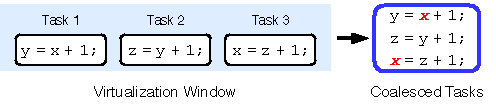
\includegraphics[width=0.8\columnwidth]{figures/coalesced-war.pdf}
	\caption{Task coalescing-induced WAR dependency (in the case of this example, at variable $x$). Such dynamic dependencies cannot be resolved at compile-time and they break memory consistency.}
	\label{figure:coalescedWar}
\end{figure}

Resolving WAR (Write-After-Read) dependencies by considering static task boundaries is not sufficient to keep non-volatile memory consistent when tasks are coalesced. Not handling WAR dependencies on a coalesced task scope introduces a new problem, which we denote as \emph{task coalescing-induced WAR dependency}. This problem is illustrated in Fig.~\ref{figure:coalescedWar}. Therefore, \sys implements novel {\em Virtual Memory Manager} (VMM) which enables task coalescing guaranteeing data integrity, which is at the same time efficient.

VMM overview is given in Fig.~\ref{figure:mem-man}.
VMM abstracts the physical address space of the non-volatile memory (FRAM) and divides it into \texttt{\underline{private}} and \texttt{\underline{shadow}} (underlined locations are non-volatile) buffers, and each buffer is divided into pages.
\texttt{\underline{private}} holds the consistent version of pages after each commit (and on reboot), while \texttt{\underline{shadow}} serves as support during the execution of coalesced tasks.
The VMM prohibits applications from directly accessing these buffers.
Instead, it redirects any request to the \texttt{working} buffer located in the volatile memory (SRAM), which has a lower latency and energy cost to access than FRAM.
It populates the \texttt{working} buffer with the privatized pages from non-volatile memory requested by tasks.
When a coalesced task completes, the VMM ensures that {\em dirty}, i.e., modified, pages are committed to FRAM and visible to subsequent tasks.
If a power failure interrupts a task, all temporary modifications to pages in \texttt{working} (and \texttt{\underline{shadow}}) occurred after the last commit are discarded in order to keep data consistency.
On a commit, the VMM atomically copies, through a two-phase commit, all dirty pages back into their location in the non-volatile memory.
% SRAM has a limited size and there is an extended working memory containing {\em shadow pages} in the larger FRAM. A shadow page stores the data from an updated page that needs to be committed back to non-volatile memory, but that exceeded the size of the volatile working memory.

\begin{figure}
    \centering
    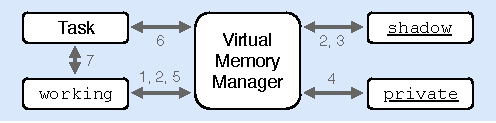
\includegraphics[width=0.8\columnwidth]{figures/mem-man.pdf}
    \caption{Interaction between task, memory manager and memory buffers upon \texttt{RP} and \texttt{WP}, and order of occurrence. Steps 2, 3, 4 and 5 are conditional.}
    \label{figure:mem-man}
\end{figure}

\subsection{Address Translation and Variable Access}

A task must access protected non-volatile variables through \sys's restricted memory interface.
The interface includes \texttt{RP}$(v)$, to read the value of variable $v$, and \texttt{WP}$(v)$ to assign a value to variable $v$.
The implementation of {\tt RP} is shown in Algorithm~\ref{algo:rwar}, and {\tt WP}'s implementation is similar except that accessed page are marked as dirty.
{\tt RP} and {\tt WP} operations translate a variable's physical address in non-volatile memory into a \emph{virtual address} in \texttt{working} in volatile memory.
In \sys, a virtual address is composed of a \emph{page tag} that identifies the page and a \emph{page offset} that identifies a byte.

\begin{algorithm}[t]
    \captionof{algorithm}{\texttt{RP}(variable $v$)}
    \label{algo:rwar}
    \small
    \begin{algorithmic}[1]
		\State $t \leftarrow \Call{GetTag}{v}$
        \State $i \gets \{ j\ |\ \Call{GetTag}{\texttt{working}[j]} = t \}$ \Comment{Search page}
		\If { $i = \emptyset$ } \Comment{Variable in a resident page?}
		\State	$i \gets \Call{PageFault}{t}$ \Comment{Swap page in}
		\EndIf
		\State $o \leftarrow \Call{GetOffset}{v}$
		\State \Return \texttt{working}[$i$][$o$]  \Comment{Return from page}
	\end{algorithmic}
\end{algorithm}

After address translation (Fig.~\ref{figure:mem-man}, Step 6), a task accesses the protected variable's location in the volatile \texttt{working} buffer (Step 7). The VMM keeps track of the page tags for the pages currently resident in the \texttt{working} buffer. When a task accesses a variable, it compares the variable's page tag to tags of the pages in {\tt working} (Algorithm~\ref{algo:rwar}, Line 2). If the accessed variable's page tag is not found in the page buffer, the operation incurs a {\em page fault} (Line 4). The byte is accessed in the page buffer at the index of the resident page and the variable's page offset (Lines 5--6).

\subsection{Page Faults and Page Swapping}

When accessing a protected variable with \texttt{RP} or \texttt{WP}, the memory manager first searches the variable's page in the \texttt{working} buffer (Fig.~\ref{figure:mem-man}, Step 1).
If the page is not found there, a page fault is incurred and a new page needs to be swapped in.
If the \texttt{working} buffer is full, a page fault on a memory access requires the VMM to swap out one of the pages in the \texttt{working} buffer (a \emph{victim page}) preserving updates made to that page.
If a task modified any byte in the victim page (i.e., using \texttt{WP}), then the page is dirty and its changes have to be persisted to non-volatile memory (Fig.~\ref{figure:mem-man}, Step 2). If the accessed page was previously modified and swapped out since the last power failure, the most recent version of the page is in {\tt \underline{shadow}} (Step 3), otherwise it has to be retrieved from {\tt \underline{private}} (Step 4). Finally, the page is copied to the volatile buffer (Step 5).

\subsection{Atomic Two-Phase Commit of Dirty Pages}

When the last task in a sequence of coalesced tasks completes, \sys must commit \emph{all} dirty pages in \texttt{working} and \texttt{\underline{shadow}}, copying them back to their original locations in \texttt{\underline{private}}. 

To make the commit atomic, \sys commits dirty pages in two phases, as shown in Algorithm~\ref{algo:commit}. The first phase copies dirty pages from \texttt{working} to the non-volatile \texttt{\underline{shadow}} (Line 4). The second phase commits pages from \texttt{\underline{shadow}} to \texttt{\underline{private}} (Line 12).  If power fails during the first phase, the whole commit is aborted, and the execution restarts from the most recently committed point (i.e., from the beginning of a coalesced task). If power fails in the second
phase, the commit process safely resumes on reboot.  The second phase depends on some run-time metadata. The \texttt{\underline{committing}} bit indicates that a commit is in progress and is set before the first page is committed (Line 9) and cleared after the last page is committed (Line 16).  The \texttt{\underline{shadowCount}} records the number of dirty shadow pages to commit and the VMM clears the counter when commit completes (Line 14). The \texttt{\underline{commitIndex}} indexes the next page to be committed (Line 11) and the VMM clears the index at the end of the phase (Line 15).

\sys's commit is efficient because it maintains an index of dirty pages instead of iterating through all potentially dirty pages to check their state.
Another source of efficiency lies in the second phase of the commit:
% \sys's implementation is also efficient because
the VMM does not copy pages from \texttt{\underline{shadow}} to \texttt{\underline{private}}, instead it swaps pointers in an indirection table that maintains the pages as a double buffer.

\paragraph{Memory Consistency.}
\sys's paging mechanism ensures that a task only ever executes using consistent protected data. During task execution, modifications to protected data do not affect the \texttt{\underline{private}} buffer, because a task reads and writes the volatile \texttt{working} buffer only, and modified pages are kept in \texttt{\underline{shadow}} until commit. A power failure erases the contents of the \texttt{working} buffer, preventing a re-executing task from observing updates from a previous execution attempt. Clearing \texttt{\underline{shadowCount}} as part of the second phase commit (Line 14) ensures that all accesses to protected variables in subsequent tasks correctly access their consistent memory locations in \texttt{\underline{private}}. This solves the coalescing-induced WAR dependency problem (see Fig.~\ref{figure:coalescedWar} again).

\begin{algorithm}[t]
	\caption{Two-phase commit}
	\label{algo:commit}
	\small
	\begin{algorithmic}[1]
        \Procedure{CommitPhase1}{} \Comment{On last coalesced task}
            \For {$i \in 0..|\texttt{working}|-1$}
                \State $t \gets \Call{Tag}{\texttt{working}[i]}$
                \State $\texttt{\underline{shadow}}[\Call{Tag}{\texttt{working}[i]}] \xleftarrow{\text{DMA}} \texttt{working}[i]$
                \State $\texttt{\underline{shadowList}}[\texttt{\underline{shadowCount}}] \gets t$
                \State $\texttt{\underline{shadowCount}} \gets \texttt{\underline{shadowCount}} + 1$
            \EndFor
            \State \Call{CommitPhase2}{}
        \EndProcedure
        \Procedure{CommitPhase2}{} \Comment{\texttt{\underline{commitIndex}} 0 on first boot}
            \State $\texttt{\underline{committing}} \gets \textbf{true}$
            \While{\texttt{\underline{commitIndex}} < \texttt{\underline{shadowCount}}}
                \State $t \gets \texttt{\underline{shadowList}}[\texttt{\underline{commitIndex}}]$
                \State \Call{commitToPrivate}{\texttt{\underline{shadow}}[t]}
                \State $\texttt{\underline{commitIndex}} \gets \texttt{\underline{commitIndex}} + 1$
            \EndWhile
            \State $\texttt{\underline{shadowCount}} \gets 0$
            \State $\texttt{\underline{commitIndex}} \gets 0$
            \State $\texttt{\underline{committing}} \gets \textbf{false}$
        \EndProcedure
        \Procedure{OnBoot}{} \Comment{Invoked on every boot}
            \If { \texttt{\underline{committing}} } \Call{CommitPhase2}{}
            \EndIf
            \State $\texttt{\underline{shadowCount}} \gets 0$, $i_\text{victim} \gets 0$
        \EndProcedure
	\end{algorithmic}
\end{algorithm}

\subsection{Dynamic Paging of \sys}

\sys asks the programmer to use its {\tt RP} and {\tt WP} API methods on every access to a protected variable (cf. Section~\ref{sec:coala_api}). These API invocations present a risk of high overhead because there is a dynamic check on every read and write. Despite the risk of per-access overhead, \sys's dynamic memory protection scheme brings several benefits over a static approach (i.e.,~\cite{alpaca}). First, the limitations of static analysis preclude some uses of pointers due to potential pointer aliasing. For example, in the presence of arbitrary pointer operations, a function call using a function pointer, or an interrupt within a task, the system cannot statically analyze the memory behavior. Second, a static approach \textit{cannot handle task coalescing}, because a protected variable's lifetime, i.e., from first use to commit, is unknown at compile-time. \sys's dynamic, per-access instrumentation supports arbitrary use of pointers and enables task coalescing.
